%%%%%%%%%%%%%%%%%%%%%%% file template.tex %%%%%%%%%%%%%%%%%%%%%%%%%
%
% This is a general template file for the LaTeX package SVJour3
% for Springer journals.          Springer Heidelberg 2010/09/16
%
% Copy it to a new file with a new name and use it as the basis
% for your article. Delete % signs as needed.
%
% This template includes a few options for different layouts and
% content for various journals. Please consult a previous issue of
% your journal as needed.
%
%%%%%%%%%%%%%%%%%%%%%%%%%%%%%%%%%%%%%%%%%%%%%%%%%%%%%%%%%%%%%%%%%%%
%
% First comes an example EPS file -- just ignore it and
% proceed on the \documentclass line
% your LaTeX will extract the file if required
\begin{filecontents*}{example.eps}
%!PS-Adobe-3.0 EPSF-3.0
%%BoundingBox: 19 19 221 221
%%CreationDate: Mon Sep 29 1997
%%Creator: programmed by hand (JK)
%%EndComments
gsave
newpath
  20 20 moveto
  20 220 lineto
  220 220 lineto
  220 20 lineto
closepath
2 setlinewidth
gsave
  .4 setgray fill
grestore
stroke
grestore
\end{filecontents*}
%
\RequirePackage{fix-cm}
%
%\documentclass{svjour3}                     % onecolumn (standard format)
%\documentclass[smallcondensed]{svjour3}     % onecolumn (ditto)
\documentclass[smallextended]{svjour3}       % onecolumn (second format)
%\documentclass[twocolumn]{svjour3}          % twocolumn
%
\smartqed  % flush right qed marks, e.g. at end of proof
%
\usepackage{graphicx}
\usepackage{varwidth}
\usepackage{setspace}
%
% \usepackage{mathptmx}      % use Times fonts if available on your TeX system
%
% insert here the call for the packages your document requires
%\usepackage{latexsym}
% etc.
%
% please place your own definitions here and don't use \def but
% \newcommand{}{}
%
% Insert the name of "your journal" with
% \journalname{myjournal}
%
\begin{document}

\title{Toward Improving Human-Robot Collaboration with Emotional Awareness}%\thanks{Grants or
% other notes about the article that should go on the front page should be
%placed here. General acknowledgments should be placed at the end of the article.}
%}

%\subtitle{Do you have a subtitle?\\ If so, write it here}

%\titlerunning{Short form of title}        % if too long for running head

\author{Mohammad Shayganfar \and
        Charles Rich \and
        Candace L. Sidner
}

%\authorrunning{Short form of author list} % if too long for running head

\institute{Mohammad Shayganfar \and Charles Rich \and Candace L. Sidner \at
              100 Institute Road, Worcester, MA, USA 01609-2280 \\
              Tel.: +1 508-831-5357\\
              Fax: +1 508-831-5776\\
              \email{mshayganfar@wpi.edu}\\
              \email{rich@wpi.edu}\\
              \email{sidner@wpi.edu}\\
%             \emph{Present address:} of F. Author  %  if needed
}

\date{Received: date / Accepted: date}
% The correct dates will be entered by the editor


\maketitle

\begin{abstract}\ldots


\keywords{Human-Robot Collaboration \and Emotion-Awareness \and Affective
Motivational Collaboration Theory}
% \PACS{PACS code1 \and PACS code2 \and more}
% \subclass{MSC code1 \and MSC code2 \and more}
\end{abstract}

\section{Introduction}
\label{intro}

- The importance of understanding collaboration.

\noindent- The importance of understanding underlying processes of the
collaboration process.

\section{Related Work}

\subsection{Emotions in Social Context}

\subsection{Social Functions of Emotions}

\subsection{Affect and Motives}

\subsection{Collaboration Theory}
\label{sec:collaboration-theory}

\section{Example Scenario}
\label{sec:example-scenario}
%Text with citations \cite{RefB} and \cite{RefJ}.

\subsection{The Backstory}

The scenario transpires in a NASA's research center. Light, temperature and
other environmental factors are simulated based on conditions on the surface of
the moon. The mission is to finish installing the required solar panels to
provide energy for the operation of NASA's science lab on the moon. Ninety
percent of these panels have already been installed. However, the operation is
now faced with low batteries which forces everyone to be cautious about
consuming energy. The astronaut is inspecting the working conditions in the
field and planning the installation of the remaining panels in collaboration
with the robot. He determines that the sun will cast shadows over the
installation structure, leading to potential difficulties. The astronaut asks
control base to go through the final checks of the robot and prepare it for the
operation.

\subsection{Astronaut-Robot Interaction}

The robot and the astronaut will collaborate with each other to achieve their
shared goal, which is to install two solar panels. They will face various
difficulties, ranging from the task being unpleasant and challenging to
conflicts of their private and/or shared goals occurring because of a blocked or
a protracted sub-task. The robot and the astronaut will go through a series of
assessment processes to figure out a) how did the current blocking happen? b)
why is the current task is blocked? and c) what is the next action they are
going to take? The robot uses its cognitive abilities and its communication
skills to overcome these problems and to motivate the astronaut to propose
alternative tasks. The following is part of an interaction between the astronaut
and the robot during their collaboration on installing solar panels.

\subsection{Agreeing on Shared Goal (Emotion-Awareness)}
\label{sec:exp1}

This and the next hypothetical examples show that agreeing on a shared goal
requires the Robot to be aware of its collaborator's emotions (here it is
frustration). In this example, the Astronaut's first turn (A1), shows her
verbally conveying her frustration with respect to the disfunctioning
measurement tool for checking the quality of the installed panel. In return, the
Robot's first turn (A2), as the crucial part of this interaction shows the Robot
perceiving the Astronaut's frustration and acknowledging that verbally. Later
on, in Section \ref{sec:wt-exp1}, we are going to show how the computational
mechanisms, discussed in Section \ref{sec:AMCT}, are involved in this process.
In other words, we are going to discuss how the emotion-driven goal-directed
mechanisms can work together and lead the Robot's behavior to acknowledge
perceived emotion of the Astronaut properly to avoid termination of the
collaboration. Continuing in turn A3, the Astronaut's utterance shows the change
of the underlying belief from termination of the collaboration to a belief
showing the possibility of seeking instrumental support by asking the Robot
whether it is possible to fix the measurement tool. Notice that the proper
acknowledgement of the Astronaut's emotion helps to change her emotion from
frustration to neutral. Now that the Astronaut does not express a negative
emotion (i.e., frustration), and she is asking for instrumental support, the
Robot can provide the alternative task as a potential solution. Here is another
advantage of the emotion-awareness in this hypothetical example. Although, the
Robot, according to the shared plan (see Sections \ref{sec:collaboration-theory}
and \ref{sec:AMCT}), could provide the same alternative task as solution to the
Astronaut, instead, it procrastinated providing the potential solution based on
the Astronaut's negative emotional state, i.e., frustration. Finally, since
agreeing on a shared goal is a collaborative negotiation process,
emotion-awareness plays an imperative role in providing a more fair offer to the
collaborator during negotiation. As a result, the Astronaut's response in the
last turn (A5) shows the acceptance of the Robot's potential solution to
continue collaboration and agreeing on the shared goal. In the next example we
are going to show what happens to the same hypothetical example when the Robot
ignores the Astronaut's emotion and tries to save the collaboration process from
failure.\\

\begin{spacing}{1.2}
\small{ 
\begin{description}
  \item \textit{\textbf{A1. Astronaut:}} Oh no! Finishing the quality check of
  our installation with this measurement problem is so frustrating. I think we
  should stop now!

  [\textit{Astronaut is frustrated.}]\\

  \item \fbox{\begin{varwidth}{0.96\textwidth}\textit{\textbf{A2. Robot:}}
  \underline{I see. This is frustrating.} But, I can help you with the
  measurement tool and we can finish the task as originally planned.

  [\textit{Robot perceives Astronaut's frustration and acknowledges that.}]
  \end{varwidth}}\\
  
  \item \textit{\textbf{A3. Astronaut:}} Can you fix the measurement tool?

  [\textit{Astronaut's emotion is neutral.}]\\
  
  \item \textit{\textbf{A4. Robot:}} The next task is fixing the panel and it
  needs you to prepare and attach the welding rod to your welding tool. To save
  our time, I will fetch another measurement tool while you are preparing your
  welding tool.

  [\textit{Robot perceives Astronaut's neutral emotion, and tries to negotiate
  and provide a fair offer.}]\\

  \item \textit{\textbf{A5. Astronaut:}} That would be great!
  
  [\textit{Astronaut is content.}]
  
\end{description}
}
\end{spacing}


\subsection{Agreeing on Shared Goal (Emotion-Ignorance)}
\label{sec:exp2}

This example shows the same process of agreeing on a shared goal as previous
one except that it diverges from reaching to an agreement, despite the fact
that it begins with the same utterance (B1) as it appears (A1) in previous
example. As mentioned earlier in Section \ref{sec:exp1}, the emotion-awareness
is beneficial in collaboration by channeling the collaboration process towards
the shared goal in the right direction. Without the emotion-awareness a
collaborative Robot will try to maintain the status of the shared goal and
prevent it from failure without considering its collaborator's negative emotion
which can be a direct result of a type of task failure during collaboration.
First, the emotion-ignorant Robot does not acknowledge the Astronaut's
frustration (i.e., B2 in compare to A2 in Section \ref{sec:exp1}), since it does
not perceive that emotion. Then, while negotiating the shared goal the Robot
fails to offer a potential solution based on the Astronaut's emotional state,
resulting in the failure of the negotiation during collaboration.

In this example, the Robot is not capable of perceiving the Astronaut's emotion,
thus it does not apply this emotion (i.e., frustration) as an influential factor
in its computational mechanisms (see Section \ref{sec:AMCT}). Hence, in the
Robot's first response to the Astronaut's utterances (B2), first it does not
acknowledge the Astronaut's emotion, and second, it immidiately conveys two
available alternative actions according to the shared plan (see Section
\ref{sec:collaboration-theory}) and asks the Astronaut to select between these
two actions. As it appears in the Astronaut's response, the Robot's immidiate
proposal does not make any progress in collaboration. As a result, the Astronaut
just repeats himself about the task status (B3) while still expresses
frustration. The Astronaut's response does not change the Robot's mental state
and this causes the Robot to try to repeat its own question (B4). The Robot's
utterance creates an ambiguious assumption for the Astronaut on whether the
Robot can fix the broken measurement tool for her. This ambiguity makes the
Astronaut even more frustrated and causes her to ask a question to remove the
ambiguity of the Robot's proposal (B5). In return, the Robot not only misses the
Astronaut's intensified frustration, but it also nullifies the Astronaut's
assumption about fixing the disfunctional measurement tool and proposes the
potentioal solution of replacing the broken tool and seeing whether the
Astronaut agrees on that (B6). In B7, the Astronaut modifies its assumption and
announces the shortage of time as justification of expressing her anger. At this
point, the Robot's response becomes more crucial since its wrong way of
interaction and emotion-ignorance behavior shift the Astronaut's emotional and
mental states into a noncollaborative status. Consequently, again, the Robot
wants to revive the collaboration process, therefore it provides more
information about the repercussions of terminating the collaboration process and
wants to see whether the Astronaut can pursue another task (B8). Finally, the
incorrect interaction of the Robot caused by its emotion-ignorance behaviors
which was developed since the Robot's very first response, leads to an
unsuccessful termination of their collaboration (B9).\\

\begin{spacing}{1.2}
\small{
\begin{description}
  \item \textit{\textbf{B1. Astronaut:}} Oh no! Finishing the quality check of
  our installation with this measurement problem is so frustrating. I think we
  should stop now!

  [\textit{Astronaut is frustrated.}]\\

  \item \fbox{\begin{varwidth}{0.96\textwidth}\textit{\textbf{B2. Robot:}} I can
  help you with the measurement tool, or we can terminate this task.
  \underline{What do you want me to do?}

  [\textit{Robot does not perceive Astronaut's frustration.}] \end{varwidth}}\\
  
  \item \textit{\textbf{B3. Astronaut:}} As I said the measurement tool does not
  work properly. We can not continue!

  [\textit{Astronaut is frustrated.}]\\
  
  \item \textit{\textbf{B4. Robot:}} Okay. Do you want me to fix this problem
  or terminate the task?

  [\textit{Robot does not perceive Astronaut's frustration.}]\\

  \item \textit{\textbf{B5. Astronaut:}} Can you fix my measurement tool?
  
  [\textit{Astronaut is frustrated, even more.}]\\
  
  \item \textit{\textbf{B6. Robot:}} I cannot fix your measurement tool, but I
  can fetch another one for you if you want?
  
  [\textit{Despite Astronaut's strong frustration, Robot tries to negotiate.}]\\
  
  \item \textit{\textbf{B7. Astronaut:}} No, I don't want another measurement tool!
  We don't have time for that!
  
  [\textit{Astronaut is angry.}]\\
  
  \item \fbox{\begin{varwidth}{0.96\textwidth}\textit{\textbf{B8. Robot:}} Okay.
  You want me to terminate this task. Terminating this task can influence the
  quality of installing this solar panel which can cause the mission to fail.
  Or, \underline{do you want us to work on another task?} This can help us to
  install the panel using your welding tool, but I do not know whether the
  quality of our installation will be acceptable.
  
  [\textit{Not only the Robot does not perceive Astronaut's anger, but also
  continues to negotiate the next step based on the shared plan to select proper
  action.}] \end{varwidth}}\\
  
  \item \textit{\textbf{B9. Astronaut:}} I told you we have this problem and we
  should terminate the mission! We cannot continue without the measurement tool!
  
  [\textit{Astronaut is angry.}]\\
  
\end{description}
}
\end{spacing}

\subsection{Delegation of a Task (Emotion-Awareness)}
\label{sec:exp3}

This and the next hypothetical examples show how delegation of a task critically
depends on understanding how worried the other collaborator is and the necessity
of having sufficient time, which play together. This example shows when the
Robot is aware of the Astronaut's worriedness, it can use its own motivation
mechanism drived by emotions to come up with a way to alleviate that. Its
methods are to exactly postpone any questions until such time as they are
critical (effects are appeared in C2, C4). At the beginning of this example
(C1), Astronaut is worried because of the lack of time in achieving the shared
goal (finishing to install solar panels) for the overall task. She proposes the
Robot to begin installing the second panel, since the first one still has some
problems. The Robot in its first turn (C2), perceives the Astronaut's emotion
(i.e., worriedness) and using the same cognitive mechanisms (see Section
\ref{sec:AMCT}) acknowledges the Astronuat's emotion just as it did in first
example in Section \ref{sec:exp1}. As mentioned earlier, we are going to show
step-by-step (see Sections \ref{sec:wt-exp1} to \ref{sec:wt-exp4}) how different
emotion-driven goal-directed mechanisms get invloved in each turn of the
collaboration process to appropriately respond to the Astronaut based on the
\textit{Affective Motivational Collaboration Theory} (see Section
\ref{sec:AMCT}). Continuing in this example, after acknowledging the Astronaut's
emotion, the Robot infers that it needs to postpone asking questions about the
missing parts of the shared plan (see Section \ref{sec:collaboration-theory})
since installing a panel is a collaborative task and some of the primitive tasks
need to be done by the Astronaut. Then, the Astronaut perceives the Robot's
response as a proper acceptance of the task delegation and tries to communicate
the status of her own, even though she is still worried about finishing the
overall task (C3). Now, the Robot without asking the actual questions, declares
the possibility of asking some follow-up questions whenever the Astronaut's
answers are required to make progress in executing some primitive tasks
while installing the second panel (C4). Here, the Robot not only prevents
overwhelming the Astronaut with several questions related to executing the next
steps in the future, but its utterance implicitly reveals its knowledge of
tasks' requirements to the Astronaut. As a result, the Robot's appraoch on
acceptance of the delegated task mitigates the Astronaut's negative emotion
(i.e., worriedness) which makes her to respond possitively to the Robot's
proposal. The next example explains the same hypothetical task delegation
scenario except it shows the negative impact of missing the Astronaut's emotion
on task delegation process.\\

\begin{spacing}{1.2}
\small{
\begin{description}
  \item \textit{\textbf{C1. Astronaut:}} I still have some problems with
  attaching the first panel! We do not have enough time. You should begin to
  install the second panel.

  [\textit{Astronaut is worried.}]\\

  \item \fbox{\begin{varwidth}{0.96\textwidth}\textit{\textbf{C2. Robot:}} Okay.
  \underline{Don't worry.} I can handle that.

  [\textit{Robot perceives Astronaut's worriedness and acknowledges that. Also,
  it doesn't ask the Astronaut (because of perceiving worriedness) if it is okay
  to leave the current task which was helping the Astronaut to install the first
  panel.}]\\
  
  [\textit{Robot perceives the Astronaut's request as on “open planning” (as
  oppose to specific executive) task delegation.}]\end{varwidth}}\\
  
  \item \textit{\textbf{C3. Astronaut:}} I will try to fix it asap.

  [\textit{Astronaut's is still worried.}]\\
  
  \item \textit{\textbf{C4. Robot:}} I might need to ask some questions while I
  am installing the second panel.

  [\textit{Robot perceives Astronaut's worriedness.}]\\

  [\textit{Robot checks a) dependencies of the task (a sub-task might need to be
  done by both parties), b) preconditions, c) required resources, d) possible
  future conflicts.}]\\
  
  [\textit{Robot needs to ask several questions to remove uncertainties, but
  because of the Astronaut's emotion, Robot decided to postpone questions about
  the details to when the Astronaut's answers are necessary to make progress.
  Robot modifies its utterance in a proper way.}]\\
  
  \item \textit{\textbf{C5. Astronaut:}} That's fine. Just let me know.
  
  [\textit{Astronaut is neutral.}]
  
\end{description}
}
\end{spacing}

\subsection{Delegation of a Task (Emotion-Ignorance)}
\label{sec:exp4}

This hypothetical example is also about task delegation (similar to the example
in Section \ref{sec:exp3}) and it shows how ignoring the collaborator's emotions can
impact the progress of a collaboration. In this example, the emotion-ignorant
Robot is doing planning in its most efficient manner (efficient because time is
short): asking a lot of questions (see utterances in D2, D4, D6, D8, D10) so
that it can work out the plan. But asking questions exacerbates the Astronaut's
worry which leads to an unsuccessful collaboration due to the lack of time.
As it is shown, the very first utterance of the Astronaut (D1) is the same as
the first utterance in previous example (C1). The Astronaut is worried and
expresses her worry. However, the Robot is not capable of perceiving and
consequently acknowledging the Astronaut's emotion. As a result, the Robot
responds to the Astronaut since the Astronaut's proposed task changes the
Robot's focus of attention to a new task, and now, the Robot tries to determine
a proper solution for an action selection problem. The reason that the Robot
perceives the Astronaut's proposal as an action selection problem is primarily
caused by the shift in the Robot's focus of attention from an unfinished
ongoing task (unsatisfied postconditions) to a new partially known nonprimitive
task (i.e., installing the second panel). Therefore, the Robot immediately tries
to confirm leaving the current unfinished task (D2). Notice the absence of
acknowledging the Astronaut's emotion by the Robot in this turn (compare C2 in
Section \ref{sec:exp3} and D2 here). This vacancy of the emotional awareness
is the beginning of the failure of the task delegaton process. As we can see,
the Robot's response does not mitigate the Astronaut's worriedness about the
future of the collaboration. Next, the Astronaut tries to help the Robot to
select the proper action by responsing possitively about the Robot leaving
the current task (D3). Now, the Robot shifts its focus of attention to the new
task and uses the Collaboration mechanism (see Section \ref{sec:AMCT}) to obtain
required information such as task dependencies, existing preconditions and
required resources as well as the existance of a plan. Subsequently, the absence
of the required information and dependencies to the Astronaut's actions causes
the Robot to ask a question about whether the Astronaut will be able to help in
some parts of the task (D4). Although, the Robot's interactive behavior is
crucial in many collaborative context, the Astronaut's worriedness caused by the
lack of time is ignored by the Robot. This ignorance of the Astronaut's
emotional state influences her mental states and consequently her behavior.
Thus, she succinctly responds to the Robot's question (D5). The Robot asks
another question about the required inputs for the task which are dependent
to the Astronaut without considering her worriedness (D6). At this point, since
the Astronaut believes that the Robot's questions are unneccessary, she becomes
frustrated and impatiently answers the Robot's question (D7). However, once
again, not only the Robot misses the Astronaut's emotion, but it also uses a
collaboration function (i.e., Reflection - see Section \ref{sec:AMCT}) to
prevent failure of a task in the future based on reflection of the same task in
similar situation in the past (D8). Then, the Astronaut does not recall the
event referenced by the Robot and since she is frustrated, she does not even
try to remove the ambiguity of the existing issue (D9). Therefore, the Robot
tries to see whether the Astronaut wants the Robot to clarify the issue for her
by providing her some examples (D10). At last, the Astronaut terminates the
collaboration task because of the lack of time (D11).\\

\begin{spacing}{1.2}
\small{
\begin{description}
  \item \textit{\textbf{D1. Astronaut:}} I still have some problems with
  attaching the first panel! We do not have enough time. You should begin to
  install the second panel.

  [\textit{Astronaut is worried.}]\\

  \item \fbox{\begin{varwidth}{0.96\textwidth} \textit{\textbf{D2. Robot:}}
  Okay. I can handle that. \underline{Is it okay if I leave the current task
  though?}

  [\textit{Robot does not perceive Astronaut's worriedness.}]\\
  
  [\textit{Robot perceives the Astronaut's request as on “open planning” (as
  oppose to specific executive) task delegation.}] \end{varwidth}}\\
  
  \item \textit{\textbf{D3. Astronaut:}} Yes, that's fine. I can finish it by my
  own.

  [\textit{Astronaut is still worried.}]\\
  
  \item \textit{\textbf{D4. Robot:}} Okay. But according to the plan, I need
  your help when we need to weld the panel. Will you be able to help me?

  [\textit{Robot does not perceive Astronaut's worriedness.}]\\

  [\textit{Robot checks a) dependencies of the task (a sub-task might need to be
  done by both parties), b) preconditions, c) required resources, d) possible
  future conflicts.}]\\
  
  [\textit{Robot needs to ask several questions to remove uncertainties, so it
  does, since it misses the Astronaut's negative emotion.}]\\
  
  \item \textit{\textbf{D5. Astronaut:}} Yes, I will.
  
  [\textit{Astronaut is more worried about finishing the first panel.}]\\
  
  \item \textit{\textbf{D6. Robot:}} We also need your welding tool and supplies
  as well as the measuring tool to install the second panel.
  
  [\textit{Robot does not perceive Astronaut's worriedness. So, it continues to
  ask question.}]\\
  
  \item \textit{\textbf{D7. Astronaut:}} Just let me know whenever you need
  something!
  
  [\textit{Astronaut becomes frustrated, since he thinks the Robot's questions
  are killing time.}]\\
  
  \item \fbox{\begin{varwidth}{0.96\textwidth} \textit{\textbf{D8. Robot:}}
  Thanks. I will. \underline{How about the conflict that might occur while I am
  trying} \underline{to fix the second panel?} You are going to need my help at
  the same time. Last time this issue terminated our mission.
  
  [\textit{Not only the Robot does not perceive Astronaut's frustration, but
  also asks about some possible future problems based on reflection of the same
  tasks in the past.}] \end{varwidth}}\\
  
  \item \textit{\textbf{D9. Astronaut:}} Robot, I really don't understand what
  you are talking about!
  
  [\textit{Astronaut becomes more frustrated.}]\\
  
  \item \fbox{\begin{varwidth}{0.96\textwidth} \textit{\textbf{D10. Robot:}}
  \underline{Do you want me to provide some examples?}
  
  [\textit{Robot does not perceive Astronaut's strong frustration. So, it
  doesn't stop asking questions.}] \end{varwidth}}\\

  \item \textit{\textbf{D11. Astronaut:}} We don't have time for this anymore!
  
  [\textit{Astronaut becomes angry.}]\\

\end{description}
}
\end{spacing}

\section{Computational Framework}
\label{sec:computational-framework}

As we mentioned in Section \ref{sec:example-scenario}, all provided examples in
Sections \ref{sec:exp1} to \ref{sec:exp4} will be discussed in more detail using
a computational theory which we call it the \textit{Affective Motivational
Collaboration Theory}. There are several mechanisms involved in our
computational framework applying different concepts of the \textit{Affective
Motivational Collaboration Theory} to provide an emotion-regulated collaborative
behavior for a robot. In this section, we are going to breifly describe all
these mechanisms without elaborating the constructing processes involved in
each mechanism since it is not in the scope of this paper. We also explain
different types of associated mental states in our computational framework based
on the \textit{Affective Motivational Collaboration Theory}.

\subsection{Affective Motivational Collaboration Theory}
\label{sec:AMCT}

\textit{Affective Motivational Collaboration Theory} is about the interpretation
and prediction of the observable behaviors in a dyadic collaborative
interaction. The theory focuses on the processes regulated by emotional states.
It aims to explain both rapid emotional reactions to events as well as
slower, more deliberative responses. These observable behaviors represent the
outcome of reactive and deliberative processes related to the interpretation of
the self's relationship to the collaborative environment. These reactive and
deliberative processes are triggered by two types of events: \textit{external}
events, such as the other's \textit{utterances} and \textit{primitive actions},
and \textit{internal} events, comprising changes in the self's mental states,
such as belief formation and emotional changes. \textit{Affective Motivational
Collaboration Theory} explains how emotions regulate the underlying processes in
the occurrence of these events during collaboration.

Emotion-regulated processes operate based on the self's mental states including
the anticipated mental states of the other, generated according to the self's
model of the other. These mental states include beliefs, intentions, goals,
motives and emotion instances. Each of these mental states possesses multiple
attributes impacting the relation between cognition and behavior or perception.

\begin{figure}[h!]
  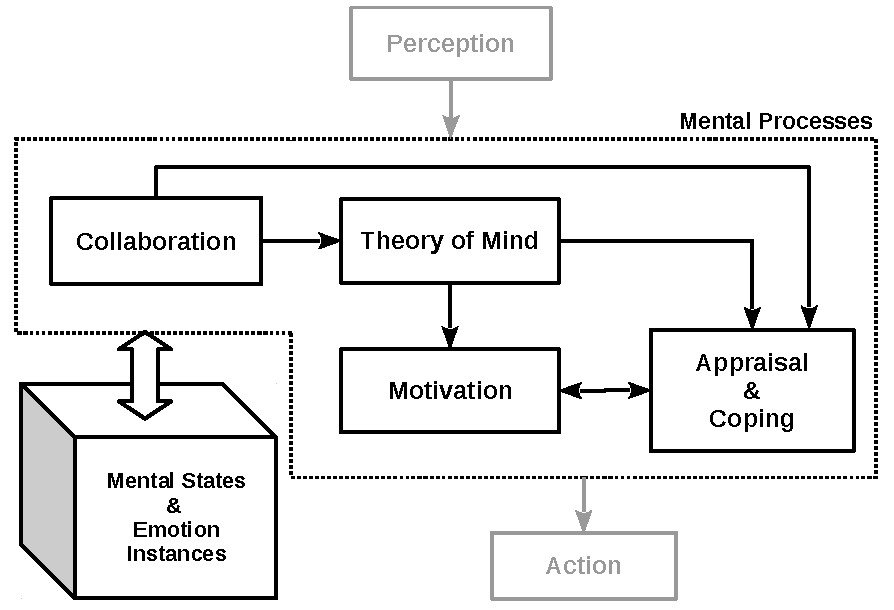
\includegraphics[scale=0.78]{figure/theory-general-croped.pdf}
  \caption{Roadmap of \textit{Affective Motivational Collaboration Theory}
  showing primary influences between processes.}
  \label{fig:theory}
\end{figure}

There are several theories which describe the underlying structure of a
collaboration based on mental states of the collaborators. The collaboration
structure of \textit{Affective Motivational Collaboration Theory} is based on
the SharedPlans theory \cite{grosz:shared-plans}. \textit{Affective Motivational
Collaboration Theory} focuses on the processes that generate, maintain and
update this structure based on mental states. The collaboration structure is
important because social robots ultimately need to co-exist with humans, and
therefore need to consider humans mental states as well as their own internal
states and operational goals.

\subsection{Underlying Mechanisms}
\label{sec:mechanisms}

The \textit{Affective Motivational Collaboration Model} consists of seven
mechanisms (see Fig.~\ref{fig:theory}) most of which directly store and
fetch the data in the Mental States.

\subsubsection{Collaboration Mechanism}

The \textit{Collaboration} mechanism (see Fig.~\ref{fig:theory}) maintains
constraints on actions. These constraints include constraints on task states and
on the ordering of tasks. The Collaboration mechanism also provides processes to
update and monitor the shared plan. These processes depend on the Appraisal
mechanism to evaluate the current Mental States with respect to the current
status of the collaboration. The self also shifts its focus of attention
according to the outcome of the Appraisal mechanism. Moreover, the Collaboration
mechanism can help the self to identify the failure of a task. The Appraisal and
Motivation mechanisms provide interpretation of task failure and the formation
of new Mental States (e.g.\,intentions) respectively. Ultimately, the Coping
mechanism allows the self to perform behavior appropriate to the current state
of the collaboration.

\subsubsection{Appraisal \& Coping Mechanism}

The \textit{Appraisal \& Coping} mechanism (see Fig.~\ref{fig:theory}) consists
of the two processes of Appraisal and Coping. The Appraisal mechanism is
responsible for evaluating changes in the self's Mental States, the anticipated
Mental States of the other, and the state of the collaboration environment.
Consequently, the Appraisal mechanism (Fig.~\ref{fig:theory}) is connected to a)
the Theory of Mind mechanism, to serve as an evaluator whenever the self applies
the Appraisal mechanism in reverse appraisal \cite{gratch:reverse-appraisal}, b)
the Collaboration mechanism, to interpret the progress and changes in the
collaboration plan and associated Mental States, c) the Motivation mechanism, to
generate and assess the self's new goal-driven motives whenever a new motive or
intention is required, e.g., following the failure of a task, and d) the
Perception mechanism, to interpret the external events from the collaboration
environment. The Coping mechanism provides the self with different coping
strategies associated with changes in the self's mental states with respect to
the state of the collaboration. In other words, the Coping mechanism produces
cognitive responses based on the appraisal patterns.

\subsubsection{Motivation Mechanism}

The \textit{Motivation} mechanism (see Fig.~\ref{fig:theory}) operates whenever
the self a) requires a new motive to overcome an internal impasse in an ongoing
task, or b) wants to provide an external motive to the other when the other
faces a problem in a task. In both cases, the Motivation mechanism uses the
Appraisal mechanism to compute attributes of the competing motives. Also, the
Motivation mechanism can serve the Theory of Mind mechanism by helping the self
to infer the motive behind the other's current action. Moreover, if there is an
impasse in accomplishing a collaborative task, the self requires a new intention
to take a new action no matter whether the self or the other is responsible for
the task. In this case, the Motivation mechanism applies the beliefs associated
with the blocked task as well as the Appraisal mechanism to generate and compare
a new set of motives related to the status of the collaboration. Only one of
these competing motives is most likely to become a new intention. The Motivation
mechanism forms a new belief and ultimately a new intention based on the winning
motive. As a result, the self can take an action based on the new intention to
sustain the collaboration progress.

\subsubsection{Theory of Mind Mechanism}

The \textit{Theory of Mind} mechanism (see Fig.~\ref{fig:theory}) is the
mechanism of inferring a model of the other's anticipated Mental States. The
self will progressively update this model during the collaboration. The
refinement of this model helps the self to anticipate the other's mental state
more accurately, which ultimately impacts the quality of the collaboration and
the achievement of the shared goal. Furthermore, the self can make inferences
about the motive (or intention) behind the other's actions using the Motivation
mechanism. This inference helps the self to update its own beliefs about the
other's mental state. In the reverse appraisal process, the self also applies
the Appraisal mechanism together with updated beliefs about the other's Mental
States to make inferences about the other's current mental state based on the
other's emotional expression. Finally, the Collaboration mechanism provides the
collaboration structure, including status of the shared plan with respect to the
shared goal and the mutual beliefs to the Theory of Mind mechanism.
Consequently, any change to the self's model of the other will update the self's
mental state.

\subsection{Mental States \& Emotion Instances}

The Mental States shown in Figure \ref{fig:theory} comprise the knowledge base
required for all the mechanisms in the overall model.

\subsubsection{Beliefs}

\textit{Beliefs} are a crucial part of the Mental States. I have two different
perspectives on categorization of beliefs. In one perspective, I categorize
beliefs based on whether they are shared or not between the collaborators. The
SharedPlans \cite{grosz:plans-discourse} theory is the foundation of this
categorization in which for any given proposition the agent may have: a) private
beliefs (the agent believes the human does not know these), b) the inferred
beliefs of the human (the agent believes the human collaborator has these
beliefs), and c) mutual beliefs (the agent believes both the self and the human
have these same beliefs and both of them believe that). From another
perspective, I categorize beliefs based on who or what they are about. In this
categorization, beliefs can be about the self, the other, or they can be about
the environment. Beliefs about the environment can be about internal events,
such as outcomes of a new appraisal or a new motivate, or external events such
as the human's offer, question or request, and general beliefs about the
environment in which the agent is situated. Beliefs can be created and updated
by different processes. They also affect how these processes function as time
passes.

\subsubsection{Intentions}

\textit{Intentions} are mental constructs directed at future actions. They play
an essential role in: a) taking actions according to the collaboration plan, b)
coordination of actions with human collaborator, c) formation of beliefs about
self and anticipated beliefs about the other, and d) behavior selection in the
Coping mechanism. First, taking actions means that the agent will intend to take
an action for primitive tasks that have gained the focus of attention, possess
active motives, have satisfied preconditions for which required temporal
predecessors have been successfully achieved. Second, intentions are involved
in action coordinations in which the human's behavior guides the agent to infer
an anticipated behavior of the human. Third, intentions play a role in belief
formation mainly as a result of the permanence and commitment inherent to
intentions in subsequent processes, e.g., appraisal of the human's reaction to
the current action and self regulation. And lastly, intentions are involved in
selecting intention-related strategies, e.g., planning, seeking instrumental
support and procrastination, which these strategies are an essential category of
the strategies in the Coping mechanism. Intentions possess a set of attributes,
e.g. \textit{Involvement, Certainty, Ambivalence} which moderate the consistency
between intention and behavior. The issue of consistency between the intentions
(in collaboration) and the behaviors (as a result of the Coping mechanism in the
appraisal cycle) is important because neither of these two mechanisms alone
provides solution for this concern.

\subsubsection{Motives}

\textit{Motives} are mental constructs which can initiate, direct and maintain
goal-directed behaviors. They are created by the emotion-regulated Motivation
mechanism. Motives can cause the formation of a new intention for the agent
according to: a) its own emotional states (how the agent feels about something),
b) its own private goal (how an action helps the agent to make progress), c) the
collaboration goal (how an action helps to achieve the shared goal), and d)
other's anticipated beliefs (how an action helps the other). Motives also
possess a set of attributes, e.g., \textit{Insistence} or \textit{Failure
Disruptiveness}. These attributes are involved in comparison of newly generated
motives based on the current state of the collaboration. Ultimately, the agent
forms or updates a belief about the winning motive in the Mental States.

\subsubsection{Goals}

\textit{Goals} help the agent to create and update its collaboration plan
according to the current private and shared goal content and structure, i.e.,
the \textit{Specificity, Proximity} and \textit{Difficulty} of the goal. Goals
direct the formation of intentions to take appropriate corresponding actions
during collaboration. Goals also drive the Motivation mechanism to generate
required motive(s) in uncertain or ambiguous situations, e.g., to minimize the
risk of impasse or to reprioritize goals. The \textit{Specificity} of goals has
two functions for the agent. First, it defines the performance standard for
evaluating the progress and quality of the collaboration. Second, it serves the
agent to infer the winner of competing motives. The \textit{Proximity} of goals
distinguishes goals according to how ``far'' they are from the ongoing task.
Proximal (or short-term) goals are achievable more quickly, and result in higher
motivation and better self-regulation than more temporally distant (or
long-term) goals. Goals can influence the \textit{Strength} of beliefs, which is
an important attribute for regulating the elicitation of social emotions. The
\textit{Difficulty} of goals impacts collaborative events and decisions in the
appraisal, reverse appraisal, motive generation and intention formation
processes. For instance, overly easy goals do not motivate; neither are people
motivated to attempt what they believe are impossible goals.

\subsubsection{Emotions}

\textit{Emotions} in Mental States are emotion instances that are elicited by
the Appraisal mechanism. The agent also keeps beliefs about these emotion
instances in the Mental States. The Belief Formation mechanism creates or
updates these beliefs about emotions. These emotion instances include the
agent's own emotions as well as the anticipated emotions of the other which are
created with the help of the processes in the Theory of Mind mechanism.

\section{Walk Through Computational Examples}

In this section, we are going to discuss how the individual computational
mechanisms (see Section \ref{sec:mechanisms}) are involved in generating the
Robot's collaborative behaviors discussed in each example in Section
\ref{sec:example-scenario}. The following four walk through examples are in the
same order as the four examples in Section \ref{sec:example-scenario}. Notice
that in emotional ignorance examples, we use the same mechanisms as in the
emotional awareness examples. These examples can demonstrate the
applicability of the \textit{Affective Motivational Collaboration Theory} in
modelling and understanding of the emotion-regulated underlying processes of a
collaboration procedure.

\subsection{Agreeing on Shared Goal (Emotion-Awareness)}
\label{sec:wt-exp1}

\subsection{Agreeing on Shared Goal (Emotion-Ignorance)}
\label{sec:wt-exp2}

\subsection{Delegation of a Task (Emotion-Awareness)}
\label{sec:wt-exp3}

\subsection{Delegation of a Task (Emotion-Ignorance)}
\label{sec:wt-exp4}

\section{Conclusion and Future Work}

- Talking about other examples that I have.

%\label{sec:2} ~\ref{sec:1}

%\paragraph{Paragraph headings} 


% For one-column wide figures use
%\begin{figure}
% Use the relevant command to insert your figure file.
% For example, with the graphicx package use
%  
\includegraphics{example.eps}
% figure caption is below the figure
%\caption{Please write your figure caption here}
%\label{fig:1}       % Give a unique label
%\end{figure}
%
% For two-column wide figures use
%\begin{figure*}
% Use the relevant command to insert your figure file.
% For example, with the graphicx package use
%  
\includegraphics[width=0.75\textwidth]{example.eps}
% figure caption is below the figure
%\caption{Please write your figure caption here}
%\label{fig:2}       % Give a unique label
%\end{figure*}
%



% For tables use
%\begin{table}
% table caption is above the table
%\caption{Please write your table caption here}
%\label{tab:1}       % Give a unique label
% For LaTeX tables use
%\begin{tabular}{lll}
%\hline\noalign{\smallskip}
%first & second & third  \\
%\noalign{\smallskip}\hline\noalign{\smallskip}
%number & number & number \\
%number & number & number \\
%\noalign{\smallskip}\hline
%\end{tabular}
%\end{table}


%\begin{acknowledgements}
%If you'd like to thank anyone, place your comments here
%and remove the percent signs.
%\end{acknowledgements}

% BibTeX users please use one of
%\bibliographystyle{spbasic}      % basic style, author-year citations
%\bibliographystyle{spmpsci}      % mathematics and physical sciences
%\bibliographystyle{spphys}       % APS-like style for physics
%\bibliography{}   % name your BibTeX data base

% Non-BibTeX users please use
%\begin{thebibliography}{}
%
% and use \bibitem to create references. Consult the Instructions
% for authors for reference list style.
%
%\bibitem{RefJ}
% Format for Journal Reference
%Author, Article title, Journal, Volume, page numbers (year)

% Format for books

%\bibitem{RefB}
%Author, Book title, page numbers. Publisher, place (year)

% etc
%\end{thebibliography}

\bibliographystyle{abbrv}
\bibliography{mshayganfar.bib}

\end{document}
% end of file template.tex

